In beiden Fällen ist die grösste Kraft, die die Strasse auf das Auto ausüben kann, die maximale Haftreibungskraft $F = \mu_\mathrm{H}\,m\,g$ (ebene Strasse, gleiche Reifen). Das Auto habe die Anfangsgeschwindigkeit $v$.

\textbf{Bremsen:} Die grösste Verzögerung ist $a = \frac{F}{m} = \mu_\mathrm{H}\,g$. Das Auto steht nach der Zeit $t = \frac{v}{a}$ still; die mittlere Geschwindigkeit ist $\frac{v}{2}$. Der Bremsweg ist
\begin{align}
 s &= \frac{v}{2}\cdot t = \frac{v^2}{2a} = \frac{v^2}{2\,\mu_\mathrm{H}\,g}
\end{align}

\textbf{Ausweichen:} Die Haftreibung liefert die Zentripetalkraft, $\frac{m\,v^2}{r} = \mu_\mathrm{H}\,m\,g$. Der kleinste Kurvenradius ist
\begin{align}
 r &= \frac{v^2}{\mu_\mathrm{H}\,g} = 2\,s
\end{align}
Um einer breiten Mauer auszuweichen, muss das Auto um \ang{90} abbiegen, bevor es die Mauer erreicht. Dafür braucht es geradeaus gemessen die Strecke $r$, also das Doppelte des Bremswegs:

\begin{center}
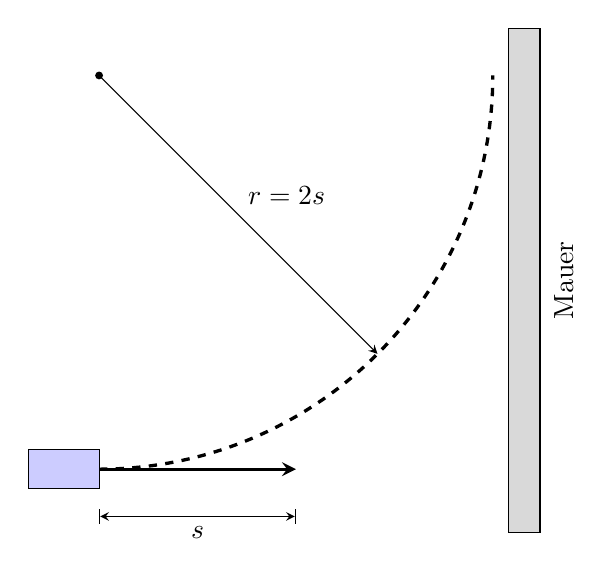
\begin{tikzpicture}[>=stealth]
 \fill[gray!30] (5.2,-0.8) rectangle (5.6,5.6);
 \draw (5.2,-0.8) rectangle (5.6,5.6);
 \node[rotate=90] at (5.9,2.4) {Mauer};
 \fill[blue!20] (-0.9,-0.25) rectangle (0,0.25);
 \draw (-0.9,-0.25) rectangle (0,0.25);
 \draw[very thick, ->] (0,0) -- (2.5,0);
 \draw[|<->|] (0,-0.6) -- (2.5,-0.6) node[midway, below] {$s$};
 \draw[very thick, dashed] (0,0) arc (-90:0:5);
 \draw[->] (0,5) -- ++(-45:5) node[pos=0.5, above right] {$r = 2s$};
 \fill (0,5) circle (0.05);
\end{tikzpicture}
\end{center}

Bremsen ist also besser: Das Auto kommt auf der halben Strecke zum Stehen. Selbst wenn der Bremsweg nicht ganz reicht, prallt es mit viel kleinerer Geschwindigkeit auf.
